\section{DevOps}

De acordo com \cite{amazon} o DevOps é a combinação de filosofias, práticas e ferramentas que aumentam a capacidade de
distribuir aplicativos e serviços em alta velocidade. Essas velocidade permite que seus clientes sejam atendidos de
forma melhor e as empresas conseguem competir de forma mais eficaz no mercado. Com esse novo modelo, as equipes de
desenvolvimento e operações não são mais separadas, ou seja, os engenheiros trabalham durante todo o ciclo de vida do
aplicativo, da fase de desenvolvimento e testes à fase de implantação e operações.

\begin{figure}[H]
	\centering
  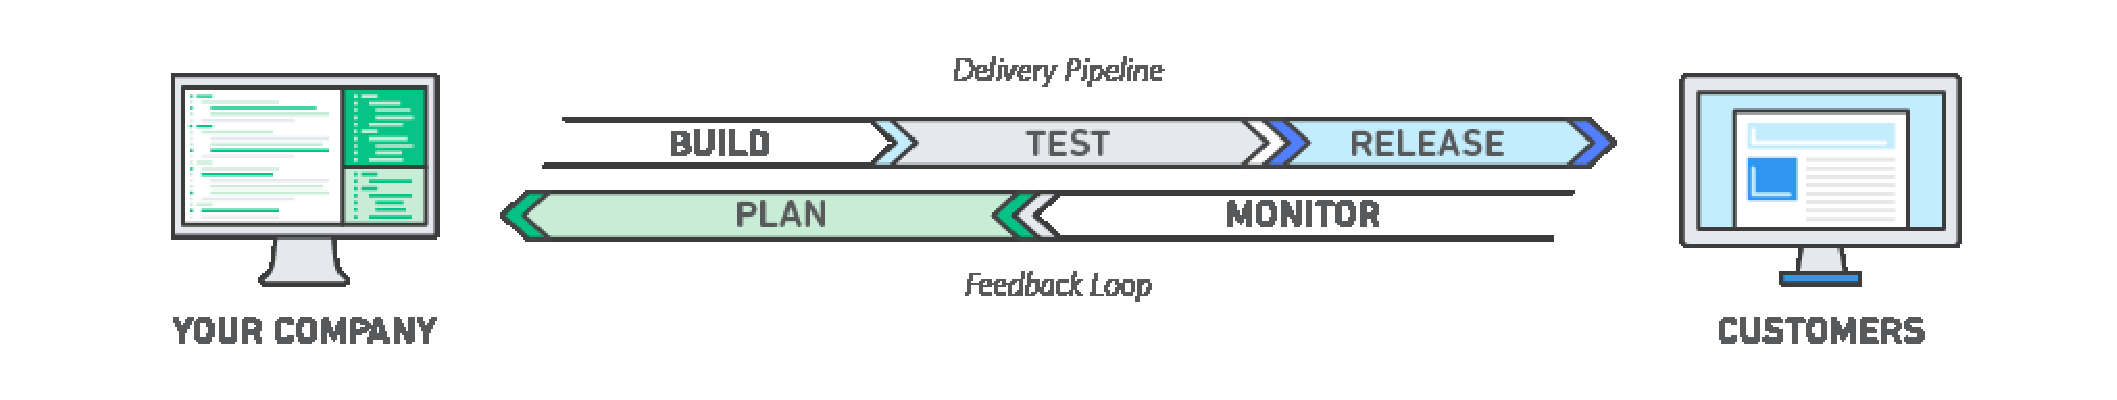
\includegraphics[keepaspectratio=true,scale=0.5]{figuras/devops_pipe.eps}
  \caption[O que é DevOps.]{O que é DevOps. Fonte: \cite{amazon}}
	\label{fig:desenvolvimento}
\end{figure}

Essas equipes usam práticas para automatizar processos que sempre foram feitas de maneira manual e lenta. Eles usam
várias técnologias que o auxiliam a automatizar todo esse processo que envolve a infraestrutura do software e isso
aumenta ainda mais a velocidade e produtividade da equipe \cite{amazon}.

A \cite{amazon} cita alguns benefícios do DevOps, são eles: velocidade, entrega rápida, confiabilidade, operações em
escala, colaboração melhorada e segurança. Além disso o modelo de DevOps é importante já que o software já não apenas
sustenta uma atividade empresarial, ele tornou-se um componente integral de cada parte de uma empresa. O objetivo
principal desse modelo é remover as barreiras entre duas equipes tradicionalmente separadas, desenvolvimento e
operações, com essa abordagem as duas equipes trabalham juntas para otimizar a produtividade dos desenvolvedores e a
confiabilidade das operações de forma a automatizar alguns processos que antes eram feitos de forma manual e que gerava
uma certa dependencia entre as equipes.

De acordo com \cite{amazon} existem algumas práticas essenciais que ajudam as empresas a inovar mais rapidamente por
meio da automação e da simplificação dos processos de desenvolvimento de software e gerenciamento de infraestrutura. A
maioria dessas práticas já são realizadas e mencionadas em algumas metodologias como o XP. São elas: integração
contínua, entrega contínua, microsserviços, infraestrutura como código, monitoramento e registro em log, comunicação e
colaboração.
